\documentclass[conference]{IEEEtran}
\usepackage{enumerate}
\usepackage{hyperref}
\usepackage{todonotes}
\usepackage[framemethod=TikZ]{mdframed}
\usepackage{graphicx}
\newmdenv [ %
 skipabove=\topsep,
 skipbelow=\topsep,
 roundcorner = 5pt,
 leftmargin = 2,
 rightmargin = 2,
 % backgroundcolor = oldlace,
 innertopmargin = 3,
 splittopskip = 3]{mq}
\ifCLASSINFOpdf
 \else
 \fi
\begin{document}

%\title{Utilizando a Fase de Empatia do Design Thinking como Facilitadora na Elicitação dos Requisitos de Privacidade
%}
\title{Using the Design Thinking Empathy Phase as a Facilitator in Privacy Requirements Elicitation}

% author names and affiliations
% use a multiple column layout for up to three different
% affiliations
%\author{\IEEEauthorblockN{Edna Dias Canedo}
%\IEEEauthorblockA{Computer Science Department, University of Bras\'{i}lia (UnB) \\
%P.O. Box 4466, Bras\'{i}lia--DF, Brazil \\
%Email: ednacanedo@unb.br}
%\and
%\IEEEauthorblockN{Angelica Toffano Seidel Calazans}
%\IEEEauthorblockA{University center -- UniCEUB\\
%Bras\'{i}lia--DF, Brazil\\
%Email: angelica.toffano@gmail.com}
%\and
%\IEEEauthorblockN{Anderson Jefferson Cerqueira}
%\IEEEauthorblockA{Computer Science Department, University of Bras\'{i}lia(UnB) \\
%P.O. Box 4466, Bras\'{i}lia--DF, Brazil \\
%Email: andersonjcdf@gmail.com}
%\and
%\IEEEauthorblockN{Pedro Henrique Teixeira Costa}
%\IEEEauthorblockA{Computer Science Department, University of Bras\'{i}lia(UnB) \\
%P.O. Box 4466, Bras\'{i}lia--DF, Brazil \\
%Email: PHTCOSTA@gmail.com} 
%\and
%\IEEEauthorblockN{Eloisa Toffano Seidel Masson}
%\IEEEauthorblockA{University center -- UniCEUB\\
%Bras\'{i}lia--DF, Brazil\\
%Email: eloisa.masson@ceub.edu.br} 
%
%}
\maketitle

\begin{abstract}
%Este artigo apresenta uma contextualização do uso da Phase de Empatia no processo de elicitação de requisitos de privacidade. Nós realizamos uma revisão de literatura para identificar o uso do da Phase de Empatia do Design Thinking na elicitação de requisitos de privacidade. Além disso, nós realizamos um survey com 63 profissionais da indústria para entender como é realizado a elicitação desses requisitos e se estes profissionais utilizam a Phase de Empatia. Nós identificamos que 73.9\% dos desenvolvedores utilizam a fase de empatia para elicitar os requisitos de software. Além disso, mais de 62\% dos profissionais da indústria não possuem conhecimento em relação aos privacy requirements, bem como em relação as ferramentas de Empatia para a requirements elicitation. Por fim, nós propomos um modelo de empatia que poderá ser utilizado pelos desenvolvedores de software no processo de elicitação dos requisitos de privacidade.%

This article presents a contextualization of the use of the Empathy Phase in the process of privacy requirements elicitation. We conducted a literature review to identify the use of the Design Thinking Empathy Phase in privacy requirements elicitation. In addition, we conducted a survey with 68 industry practitioners to understand how these requirements are elicited and whether these practitioners use the Empathy Phase. We found that 73.9\% of developers use the empathy phase to software requirements elicitation. In addition, more than 61\% of industry practitioners are unaware of privacy requirements, as well as empathy tools for requirements elicitation. Finally, we propose an empathy model that can be used by software developers in the process of privacy requirements elicitation.

\end{abstract}
\IEEEpeerreviewmaketitle

\section{Introduction}

%Com o surgimento de novas tecnologias e legislações, a proteção dos dados dos usuários precisa ser considerada durante todo o processo de desenvolvimento de software. Para implementar uma funcionalidade de um software que irá fazer uso de dados pessoais, é necessário que seja considerado os requisitos de privacidade durante a fase de elicitação de requisitos \cite{DBLP:conf/wer/NettoPS19}. A General Data Protection Regulation (GDPR) \cite{Eu2019} e a Brazilian General Data Protection Law (LGPD) \cite{leiLGPD} são leis que definem a proteção dos dados pessoais, e nas quais, fica evidente que os usuários têm o direito de receber as informações de forma clara e precisa sobre como seus dados serão tratados \cite{DBLP:conf/re/Ayala-RiveraP18}. Assim, garantir a privacidade dos dados dos usuários se tornou uma das principais preocupações no desenvolvimento de software, seja para satisfazer as necessidades dos usuários ou para cumprir as leis de privacidade em vigor \cite{DBLP:conf/sbes/PeixotoS18}, \cite{DBLP:conf/wer/NettoPS19}, \cite{DBLP:conf/amcis/HuthM19}, \cite{DBLP:conf/IEEEares/HorakSH19}.

With the advent of new technologies and legislation, the protection of users' data needs to be considered throughout the software development process. To implement software functionality that will make use of personal data, it is necessary to consider the privacy requirements during the requirements elicitation phase \cite{DBLP:conf/wer/NettoPS19}. The General Data Protection Regulation (GDPR) \cite{Eu2019} and the Brazilian General Data Protection Law (LGPD) \cite{leiLGPD} are laws that define the protection of personal data, and in which, it is evident that users have the right to receive information clearly and accurately about how your data will be treated \cite{DBLP:conf/re/Ayala-RiveraP18}. Thus, ensuring the privacy of users' data has become one of the main concerns in software development, either to satisfy users' needs or to comply with the privacy laws in force \cite{DBLP:conf/sbes/PeixotoS18},\cite{DBLP:conf/wer/NettoPS19}, \cite{DBLP:conf/amcis/HuthM19}, \cite{DBLP:conf/IEEEares/HorakSH19}.

%Os dados dos usuários devem ser protegidos antes do seu armazenamento e quando os sistemas de software apresentarem informações oriundas da análise dos dados dos usuários que foram coletados, o software deve utilizar proteções que não permitam a restauração de informações (identificação do proprietário do dado), ou seja, o armazenamento não deve permitir a restauração dos dados após a aplicação de uma solução de privacidade \cite{Eu2019},\cite{leiLGPD}. Existem diversas soluções propostas para a proteção da privacidade dos dados do usuário, dentre essas soluções, as que modificam atributos; e as que não modificam os atributos \cite{DBLP:journals/iotj/Vergara-Laurens17}.

User data must be protected before storage and when software systems present information from the analysis of user data that has been collected, the software must use protections that do not allow the restore of information (identification of the data owner), that is, storage should not allow data to be restored after the application of a privacy solution \cite{Eu2019},\cite{leiLGPD}. There are several solutions proposed to protect the privacy of user data, among these solutions, those that modify attributes; and those that do not modify the attributes \cite{DBLP:journals/iotj/Vergara-Laurens17}.

%As soluções que modificam os atributos compreendem técnicas que aplicam algoritmos para agrupar, ofuscar, anonimizar, minimizar, dentre outras, alterando a estrutura dos dados para impedir a identificação de um indivíduo no grupo. As soluções que não modificam os atributos são técnicas que aplicam algoritmos de proteção sem alteração das informações, tais como encriptação, criptografia homomórfica, etc. \cite{DBLP:journals/iotj/Vergara-Laurens17}.

The solutions that modify the attributes include techniques that apply algorithms to group, obfuscate, anonymize, minimize, among others, changing the data structure to prevent the identification of an individual in the group. Solutions that do not modify attributes are techniques that apply protection algorithms without changing information, such as encryption and homomorphic encryption  \cite{DBLP:journals/iotj/Vergara-Laurens17}.

%Desenvolver sistemas de software que garantem a proteção dos dados pessoais é um desafio para os desenvolvedores de software, tornando-se mais complexo quando envolvem sistemas distribuídos, que podem possuir diversas formas de coleta de dados dos usuários, como ocorre na maioria das aplicações comerciais e ou governamentais. Além disso, a proteção dos dados é essencial para obter a confiança e a participação dos usuários no processo de coleta de dados. Para atender a essa necessidade de proteção de dados, é preciso adotar e utilizar novas técnicas e ferramentas para elicitar os requisitos e analisar e disponibilizar os dados pessoais. Uma maneira de facilitar o processo de elicitação de requisitos de privacidade pode ser o uso do mapa de empatia \cite{DBLP:conf/sbes/FerreiraCB15} e do Design Thinking \cite{DBLP:books/lib/brown2009change}, \cite{DBLP:conf/hci/CanedoC18}.

Developing software that guarantee the protection of personal data is a challenge for software developers, becoming more complex when they involve distributed systems, which can have different ways of collecting data from users, as it happens in most commercial applications and or governmental. In addition, data protection is essential to obtain users' trust and participation in the data collection process. To meet this need for data protection, it is necessary to adopt and use new techniques and tools to requirements elicitation and analyze and make personal data available. One way to facilitate the process of privacy requirements elicitation may be to use the empathy map \cite{DBLP:conf/sbes/FerreiraCB15} and Design Thinking \cite{DBLP:books/lib/brown2009change}, \cite{DBLP:conf/hci/CanedoC18}.

%Assim, o objetivo desta pesquisa é identificar como a fase de Empatia do Design Thinking pode ser utilizada como ferramenta facilitadora na elicitação dos requisitos de privacidade. Altogether, in this work we answer questions related to (a) a utilização da fase de empatia do Design Thinking na elicitação dos requisitos de privacidade and (b) as ferramentas que podem ser utilizadas na fase de empatia para elicitar os requisitos de privacidade de uma maneira mais clara e eficaz. Accordingly, we present the following contributions:

The aim of this research is to identify how the Design Thinking Empathy phase can be used as a facilitating tool in privacy requirements elicitation. Altogether, in this work we answer questions related to (a) the use of the Design Thinking empathy phase in privacy requirements elicitation and (b) the tools that can be used in the empathy phase to elicit the privacy requirements of a company clearer and in a more effective way. Accordingly, we present the following contributions:

\begin{itemize}
    %\item \textcolor{red}{62.9\% dos desenvolvedores da indústria não possuem conhecimento sobre privacy requirements. 27.4\% afirmaram que conhecem sobre privacy requirements e 9.7\% conhecem e trabalham atualmente com a privacy requirements elicitation};
    \item 61.8\% of industry developers are unaware of privacy requirements. 26.5\% said they know about privacy requirements and 11.8\% know and currently work with privacy requirements elicitation;
    %\item  \textcolor{red}{A fase do Design Thinking mais impactante para a privacy requirements elicitation, de acordo com os desenvolvedores de software, é a fase de Emphatia com 65.4\%};
    \item  The most impactful phase of Design Thinking for privacy requirements elicitation, according to software developers, is the Empathy phase with 38.0\%;
     %\item \textcolor{red}{Os desenvolvedores acreditam que a fase de empatia pode motivar os participantes no processo de privacy requirements elicitation, embora a maioria deles não conheçam as ferramentas existentes.}
    \item The developers believe that the empathy phase can motivate participants in the privacy requirements elicitation process, although most of them are unaware of the existing tools.
\end{itemize}

%Este artigo está organizado como segue. Na Seção \ref{back} é apresentado uma contextualização sobre os principais conceitos relacionados a essa pesquisa, bem como os trabalhos correlatos. Na Seção \ref{method} é apresentada a metodologia utilizada para conduzir este trabalho. Na Seção \ref{empathy} é apresentado os resultados do survey realizado para compreender a percepção dos desenvolvedores de software do uso da Empatia e do Design Thinking na elicitação dos requisitos de privacidade. As ameaças para a validação dessa pesquisa são apresentadas na Seção \ref{thread}. Por fim, as conclusões e trabalhos futuros são apresentados na Seção \ref{conclusion}.

This article is organized as follows. In the section \ref{back} a contextualization is presented about the main concepts related to this research, as well as related works. Section \ref{method} presents the methodology used to conduct this work. Section \ref{empathy} presents the results of the survey carried out to understand the perception of software developers of the use of Empathy phase of Design Thinking in privacy requirements elicitation. The threats to validate this research are presented in Section \ref{thread}. Finally, the conclusions and future work are presented in Section \ref{conclusion}.

\section{Background}
\label{back}
\subsection{Design Thinking}

%O Design Thinking considera que a tarefa mais importante ao iniciar um projeto de desenvolvimento de software é entender as necessidades dos usuários, investigando quais são as suas necessidades e qual impacto o software causaria com o seu uso. Todos os participantes do processo de desenvolvimento procuram entender o universo do usuário com o objetivo de obter as informações necessárias para a elicitação dos requisitos e as percepções dos usuários em relação a elas \cite{DBLP:books/lib/brown2009change}. Assim, a ideia principal do Design Thinking é como os designers progridem com o processo de desenvolvimento, com ideias criativas para as soluções propostas, no intuito de descobrir e oferecer novas oportunidades \cite{DBLP:conf/hci/AdikariMC13}. O Design Thinking dissemina a inovação centrada no usuário, de modo que exista colaboração, interação e abordagens práticas para encontrar as ideias mais apropriadas e, consequentemente, soluções coerentes para os problemas dos usuários \cite{DBLP:books/lib/brown2009change}. 

Design Thinking considers that the most important task when starting a software development project is to understand the needs of users, investigating what are their needs and what impact the software would cause with its use. All participants in the development process seek to understand the user's universe in order to obtain the necessary information to requirements elicitation and users' perceptions of them \cite{DBLP:books/lib/brown2009change}. Thus, the main idea of Design Thinking is how designers progress with the development process, with creative ideas for the proposed solutions, in order to discover and offer new opportunities \cite{DBLP:conf/hci/AdikariMC13}. Design Thinking disseminates user-centered innovation, so that there is collaboration, interaction and practical approaches to find the most appropriate ideas and, consequently, coherent solutions to users' problems \cite{DBLP:books/lib/brown2009change}.

\subsubsection{Phases of Design Thinking}

%No contexto de Engenharia de Software, existem diversos modelos de Design Thinking com diferentes stages. Os modelos propostos por Sandino et al. \cite{DBLP:conf/hci/SandinoMV13}, Hiremath e Sathiyam \cite{DBLP:conf/interact/HiremathS13} and Coutinho et al. \cite{DBLP:conf/eatis/CoutinhoGJ16} apresentam sete fases. De Paula e Araújo \cite{DBLP:conf/hci/PaulaA16} propuseram um modelo de Design Thinking de seis fases associado ao processo de desenvolvimento ágil e Lean Startup. 

In the context of Software Engineering, there are several Design Thinking models with different phases. The models proposed by Sandino et al. \cite{DBLP:conf/hci/SandinoMV13}, Hiremath e Sathiyam \cite{DBLP:conf/interact/HiremathS13} and Coutinho et al. \cite{DBLP:conf/eatis/CoutinhoGJ16} have seven phases. De Paula and Ara\'{u}jo \cite{DBLP:conf/hci/PaulaA16} proposed a six-phase Design Thinking model associated with the agile development process and Lean Startup.

%Newman et al. \cite{DBLP:conf/icse/NewmanFSFFW15} apresentaram o DrivingBoard, um modelo de Design Thinking de 6 fases que utiliza Design Participativo e Desenvolvimento Ágil. Ximenes et al.  \cite{DBLP:conf/hci/XimenesAA15} combinaram Design Thinking, Lean Startup e Desenvolvimento Ágil. O Design Thinking utilizado pelos autores foi o modelo proposto pela Stanford University’s D-School e neste trabalho nós iremos utilizar esse modelo, o qual possui 5 fases, dentre elas a fase de empatia \cite{DBLP:conf/hci/XimenesAA15}, conforme apresentado na Figura \ref{fig:design_thinking_phases}: 

Newman et al. \cite{DBLP:conf/icse/NewmanFSFFW15} presented the DrivingBoard, a six-phase Design Thinking model that uses Participatory Design and Agile Development. Ximenes et al.  \cite{DBLP:conf/hci/XimenesAA15} combined Design Thinking, Lean Startup and Agile Development. The Design Thinking used by the authors was the model proposed by Stanford University's D-School and in this work we will use this model, which has 5 phases, among them the empathy phase \cite{DBLP:conf/hci/XimenesAA15}, as shown in Figure \ref{fig:design_thinking_phases}:

\begin{enumerate}

%\item Empatia: Esta fase é primordial para obter uma visão geral do usuário. É uma fase de conhecimento sobre as  necessidades e desejos dos usuários. A empatia é usada para ouvir, ver e sentir. É perceber o usuário, colocar-se no lugar dele e enxergar o quê, como e quando uma ação é possível em busca de uma solução para o problema.

\item Empathize: This phase is essential to obtain an overview of the user. It is a phase of knowing about users' needs and desires. Empathy is used to hear, see and feel. It means perceiving the user, putting himself in his place and seeing what, how and when an action is possible in search of a solution to the problem.

%\item Definição: Esta etapa talvez seja uma das mais desafiadoras, uma vez que envolve a interpretação de todos os fatos adquiridos no processo de empatia. Para que uma definição do problema seja atingida, é preciso processar tudo o que foi dito e visto na etapa de Empatia, o que pode ser uma atividade bastante trabalhosa e demorada.

\item Define: This stage is perhaps one of the most challenging, as it involves the interpretation of all the facts acquired in the process of empathy. For a definition of the problem to be reached, it is necessary to process everything that was said and seen in the Empathy phase, which can be a very laborious and time-consuming activity.

%\item Ideação: É uma fase muito abrangente, na qual as ideias e os conceitos são gerados com o objetivo de gerar inovações sobre os problemas identificados na etapa de Empatia e Definição.

\item Ideate: It is a in-depth phase, in which ideas and concepts are generated with the aim of generating innovations on the problems identified in the Empathy and Definition phase.

%\item Prototipação: Nesta fase se faz necessário construir protótipos para as ideias aprovadas. A principal função desses protótipos é permitir um teste rápido de uma ideia tangível, mesmo que seja de baixa fidelidade. Os protótipos permitem um feedback rápido dos usuários e são rápidos de fabricar, além de baratos.

\item Prototype: At this stage it is necessary to build prototypes for the approved ideas. The main function of these prototypes is to allow a quick test of a tangible idea, even if it is of low accuracy. Prototypes allow quick feedback from users and are quick to manufacture, as well as inexpensive.

%\item Teste: Esta é a última fase, sendo a hora de apresentar os protótipos criados ao usuário e buscar feedback. Essa etapa serve para refinar ideias e soluções. Os protótipos são avaliados com a prospectiva dos usuários finais para investigar se as ideias e os pressupostos manifestados nestes protótipos são consideradas soluções adequadas. Cada rodada de teste também é empática, pois as equipes aprendem muito observando como os usuários interagem com o produto. A diferença é que o teste faz com que a equipe de desenvolvimento ofereça necessariamente uma versão do produto (seja em papel, código ou qualquer outro meio aplicável) para o usuário interagir. Os testes reduzem os confrontos dentro da equipe. Isso deixa claro o que funciona melhor para o usuário. Os testes para um projeto de software criativo são muito parecidos com a engenharia de requisitos na metodologia ágil, ou seja, o usuário escolhe o que prefere. As equipes devem ser treinadas para entender quando estão fazendo hipóteses e assumindo coisas que deveriam ser testadas. 

\item Test: This is the last phase, being the time to present the prototypes created to the user and seek feedback. This step serves to refine ideas and solutions. Prototypes are evaluated with the perspective of end users to investigate whether the ideas and assumptions expressed in these prototypes are considered proper solutions. Each test round is also empathetic, as teams learn a lot by watching how users interact with the product. The difference is that the test makes the development team necessarily offer a version of the product (whether on paper, code or any other way) for the user to interact. Tests reduce clashes within the team. This makes it clear what works best for the user. The tests for a creative software project are very similar to the requirements engineering in the agile methodology, where the user chooses what he prefers. Teams must be trained to understand when they are making assumptions and assuming things that should be tested.

\end{enumerate}

\begin{figure}[!htb]
    \centering
    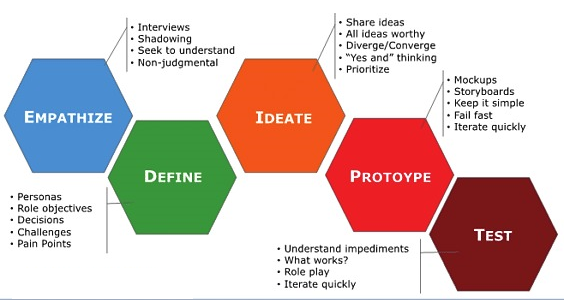
\includegraphics[width=3.4in]{Figures/FigDR.png}
    \caption{Stanford’s d.school Design Thinking and its Phases \cite{DBLP:conf/hci/XimenesAA15},\cite{ DBLP:conf/icse/CarrollR16}}
    \label{fig:design_thinking_phases}
\end{figure}

%Algumas ferramentas de apoio ao Design Thinking na fase de elicitação de requisitos são: \href{http://www.smaply.com}{Smaply}: ferramenta de persona e outros métodos tais como stakeholder map e customer journey maps; \href{http://www.stakeholder-management.com/}{Stakeholder Circle}: ferramenta de stakeholder maps; \href{http://www.touchpointdashboard.com}{Touchpoint  Dashcboard}: ferramenta de customer journey maps; \href{http://www.creately.com}{Creately}: ferramenta de service blueprint; \href{http://www.strategyzer.com}{Strategyzer}: ferramenta de business model innovation; \href{http://www.axure.com/}{Axure RP}: ferramenta de prototipação rápida.

Some tools to support Design Thinking in the requirements elicitation phase: \href{http://www.smaply.com}{Smaply}: persona tool and other methods such as stakeholder map and customer journey maps; \href{http://www.stakeholder-management.com/}{Stakeholder Circle}: stakeholder map tool; \href{http://www.touchpointdashboard.com}{Touchpoint Dashcboard}: customer journey maps tool; \href{http://www.creately.com}{Creately}: blueprint service tool; \href{http://www.strategyzer.com}{Strategyzer}: business model innovation tool; \href{http://www.axure.com/}{Axure RP}: Rapid prototyping tool.

\subsection{Empathy}

%Levy and Hadar \cite{DBLP:conf/re/LevyH18} reforçam a necessidade de empatia com os usuários finais afirmando que essa é uma habilidade de engenharia de requisitos tão necessária quanto o conhecimento técnico e a competência social. A empatia é necessária para trabalhar com a diversidade de usuários, permitindo uma melhor elicitação de requisitos. Segundo Levy and Hadar \cite{DBLP:conf/re/LevyH18}, a empatia é o primeiro passo do Design Thinking, e tem despertado interesse entre as organizações de desenvolvimento de software por alavancar os processos de design e inovação e por possibilitar uma melhor experiência para o usuário final. O Design Thinking coloca o usuário em papel de destaque, e enfatiza a construção da empatia com os usuários, observando seu comportamento e obtendo conclusões sobre o que os usuários querem e precisam. Este trabalho apresenta resultados preliminares de uma colaboração entre estudantes de design e estudantes de engenharia da Shenkar College of Engineering, Design e art. As descobertas mostram como os estudantes de engenharia, ao lidar com um ser humano praticaram empatia e usaram uma linguagem emocional na Elicitação de Requisitos para as suas soluções propostas. A experiência de aprendizado multidisciplinar de estudantes de engenharia e design, adquirida ao usar o Design Thinking pode promover empatia e outras habilidades necessárias na cultura digital moderna, devido a confluência de tecnologia, conhecimento e cultura.

Levy and Hadar \cite{DBLP:conf/re/LevyH18} reinforce the need for empathy with end users by stating that this is a requirement engineering skill as necessary as technical knowledge and social competence. Empathy is necessary to work with the diversity of users, allowing a better requirements elicitation. According to Levy and Hadar \cite{DBLP:conf/re/LevyH18}, empathy is the first step of Design Thinking, and it has aroused interest among software development organizations for leveraging design and innovation processes and for enabling better experience for the end user. Design Thinking puts the user in a prominent role, and emphasizes building empathy with users, observing their behavior and drawing conclusions about what users want and need. This work presents preliminary results of a collaboration between design students and engineering students at Shenkar College of Engineering, Design and art. The findings show how engineering students, when dealing with a human being, practiced empathy and used emotional language in Requirement Elicitation for their proposed solutions. The multidisciplinary learning experience of engineering and design students gained from using Design Thinking can promote empathy and other skills needed in modern digital culture, due to the confluence of technology, knowledge and culture.

%No contexto da Empatia versus Design Thinking, Gasparini \cite{Gasparini} abordou a Empatia explorando dois aspectos principais: a empatia emocional e a empatia cognitiva. Empatia emocional ou afetiva refere-se a uma resposta emocional compartilhada por dois ou mais individuos, por exemplo, sentimento de medo ou excitação. A empatia cognitiva está relacionada à capacidade do indivíduo de descobrir o que acontece na mente do outro, ou seja, conseguir entender o ponto de vista do outro \cite{Newkimbell}. Gasparini \cite{Gasparini} realizou um estudo de caso, para abordar a intersecção entre Design Thinking e Empatia, e apresenta os resultados de um workshop organizado pela Norwegian University Library addressing Open Access services. As metodologias e técnicas utilizadas foram a Fotoetnografia, Anotações AO vivo, User journey, Touch points and Service Design Cards. User journey is the representation of all the steps a customer need to perform to achieve the final goal of the service. Each situation where the user is in direct contact with the service provider is called a touch point. Using Service Design Cards one can make the aforementioned journey, where each card is a touch point. Gasparini \cite{Gasparini} concluiu que o uso da empatia emocional e cognitiva no processo de design apresenta bons resultados, mas que esse assunto, necessita ainda ser pesquisado, objetivando melhorar o entendimento de como essas dimensões de empatias podem ser utilizadas para obter uma percepção mais adequada das necessidades do usuário.

In the context of Empathy versus Design Thinking, Gasparini \cite{Gasparini} approached Empathy by exploring two main aspects: emotional empathy and cognitive empathy. Emotional or effective empathy refers to an emotional response shared by two or more individuals, for example, feelings of fear or excitement. Cognitive empathy is related to the individual's ability to discover what happens in the other's mind to be able to understand the other's point of view \cite{Newkimbell}. Gasparini \cite{Gasparini} conducted a case study to address the intersection between Design Thinking and Empathy, and presents the results of a workshop organized by the Norwegian University Library addressing Open Access services. The methodologies and techniques used were Photoetnography, Live Notes, User journey, Touch points and Service Design Cards. User journey is the representation of all the steps a customer need to perform to achieve the final goal of the service. Each situation where the user is in direct contact with the service provider is called a touch point. Using Service Design Cards one can make the aforementioned journey, where each card is a touch point. Gasparini \cite{Gasparini} concluded that the use of emotional and cognitive empathy in the design process has good results, but that this subject still needs to be researched, aiming to improve the understanding of how these dimensions of empathy can be used to obtain a perception best suited to the user's needs.

%Outra técnica relacionada à empatia é o Empathy Map (EM). Ele é uma técnica que auxilia no design de modelos de negócios de acordo com as perspectivas dos usuários. O Mapa de Empatia permite um melhor entendimento do ambiente, comportamento, aspirações e preocupações de um usuário \cite{DBLP:conf/hci/FerreiraBC16}. Assim, é possível realizar o levantamento de requisitos implícitos \cite{DBLP:conf/re/LevyH18}.

Another technique related to empathy is the Empathy Map (EM). It is a technique that assists in the design of business models according to the users' perspectives. The Empathy Map allows a better understanding of a user's environment, behavior, aspirations and concerns \cite{DBLP:conf/hci/FerreiraBC16}. Thus, it is possible to carry out the survey of implicit requirements \cite{DBLP:conf/re/LevyH18}.

\subsection{Privacy Requirements}

%A privacidade se tornou uma das principais preocupações no desenvolvimento de software devido à dados relativos à exploração não autorizada de dados, uso indevido de informações armazenadas em sistemas, sites de mídia social, dados da Internet e divulgação de informações pessoais a terceiros \cite{DBLP:conf/wer/2019}. Por isso, ao desenvolver novos sistemas tem-se observado a necessidade de utilizar técnicas para efetuar a elicitação de requisitos de privacidade. Vários métodos podem ser encontrados na literatura, mas neste trabalho serão listados três: Privacy-Friendly System Design, PriS e LINDDUN \cite{DBLP:conf/IEEEares/Beckers12}.

Privacy has become a major concern in software development due to data relating to unauthorized exploitation of data, misuse of information stored on systems, social media sites, internet data and disclosure of personal information to third parties \cite{DBLP:conf/wer/2019}. Therefore, when developing new systems, there is a need to use techniques to privacy requirements elicitation. Several methods can be found in the literature, but in this work four will be listed: Privacy-Friendly System Design, PriS and LINDDUN \cite{DBLP:conf/IEEEares/Beckers12} and a method proposed by Islam et al \cite{DBLP:journals/tcc/IslamOKMG18}.

%O método PriS contém uma abordagem formal para modelagem de objetivos e seu relacionamento como um gráfico. Este método formal resulta em um conjunto de processos afetados pelas metas de privacidade.

The PriS method contains a formal approach for modeling of goals and their relationship as a graph. This formal method results in a set of affected processes by the privacy goals.

The LINDDUN method is the acronym of the threats linkability, identifiablitiy, non-repudiation, detectability, information disclosure, content unawareness, and policy/consent noncompliance.

%O método Privacy-Friendly System Design, propõe uma análise de requisitos de privacidade utilizando  expectativas importantes das partes interessadas e elementos do fluxo de informações: armazenamento de dados, processamento de dados e transferência de dados, provocando preocupações com a privacidade para a coleta e armazenamento de dados pessoais, uso não autorizado dos dados pessoais coletados, acesso não autorizado a dados pessoais, erros em dados pessoais, combinação de dados pessoais de várias fontes.

The Privacy-Friendly System Design method proposes an analysis of privacy requirements using important expectations of stakeholders and elements of the information flow: data storage, data processing and data transfer, causing privacy concerns for collection and storage in
personal data, unauthorized use of the personal data collected,
unauthorized access to personal data, errors in personal data,
combination of personal data from various sources.

%Islam et. al \cite{DBLP:journals/tcc/IslamOKMG18} propõe a adoção de um método que consiste em três atividades iterativas: análise organizacional, análise de requisitos de segurança e privacidade, análise de segurança e garantia de privacidade.

Islam et. al \cite{DBLP:journals/tcc/IslamOKMG18} proposes the adoption of a method consisting of three iterative activities: organizational analysis, analysis of security and privacy requirements, security analysis and privacy guarantee.

\subsection{Related works}

%Considerando o contexto de empatia e desenvolvimento de software, Akgun et al. \cite{DBLP:journals/iam/AkgunKCD15} estudaram a empatia coletiva como uma propriedade que fornece aos membros da equipe a capacidade de identificar e trabalhar com as emoções sentidas/expressas como resultado de interações em grupo. Testaram o papel da empatia coletiva na eficácia do processo do projeto. Os autores estudaram 122 projetos de desenvolvimento de software, e descobriram que a confiança baseada em cognição, a comunicação formal dentro da equipe e a familiaridade dos membros da equipe pode influenciar a empatia coletiva das equipes de projeto. Descobriram que a empatia coletiva afeta a velocidade da equipe de comercialização do produto e o  aprendizado, e resulta em menores custos de desenvolvimento de projetos \cite{DBLP:journals/iam/AkgunKCD15}. 

Considering the context of empathy and software development, Akgun et al. \cite{DBLP:journals/iam/AkgunKCD15} studied collective empathy as a property that provides team members with the ability to identify and work with emotions felt/expressed as a result of group interactions. They tested the role of collective empathy in the effectiveness of the project process. The authors studied 122 software development projects, and found that cognition-based trust, formal communication within the team, and the familiarity of team members can influence the collective empathy of the project teams. They found that collective empathy affects the speed of the product marketing team and learning, and results in lower project development costs \cite{DBLP:journals/iam/AkgunKCD15}.

%Foi identificado somente um trabalho que pesquisa a fase da empatia do Design Thinking como facilitadora da elicitação de requisitos de privacidade. Levy and Hadar \cite{DBLP:conf/re/LevyH18} analisaram a empatia como técnica do Design thinking, identificando que os desenvolvedores de software, em geral, não se preocupam com os requisitos de privacidade. A análise desses autores demonstra que a ausência de empatia pode levar à negligência de aspectos importantes de privacidade ao projetar sistemas de software. Os autores afirmam também que a etapa da empatia, no contexto do Design Thinking, é um componente necessário para que a engenharia de requisitos possa elicitar e tratar requisitos com alto risco de serem ignorados. Além disso, a utilização de técnicas e ferramentas de empatia fornecidas pelo Design thinking podem promover uma comunicação mais estreita e a construção de  habilidades de empatia para os engenheiros de software.

Only one study was identified that researches the empathy phase of Design Thinking as a facilitator in privacy requirements elicitation. Levy and Hadar \cite{DBLP:conf/re/LevyH18} analyzed empathy as a technique of Design thinking, identifying that software developers, in general, are not concerned with privacy requirements. The analysis of these authors shows that the absence of empathy can lead to the neglect of important aspects of privacy when designing software systems. The authors also state that the empathy phase, in the context of Design Thinking, is a necessary component so that requirements engineering can elicit and deal with requirements with a high risk of being ignored. In addition, the use of empathy techniques and tools provided by Design thinking can promote closer communication and the building of empathy skills for software engineers.

%Porém é possível encontrar trabalhos relevantes que abordam sobre a elicitação de requisitos e a empatia de uma maneira geral. Para melhorar a elicitação de requisitos e a experiência de uso do software foi criada a técnica PATHY (Personas empATHY)\cite{DBLP:conf/sbes/FerreiraCB15}. Essa técnica integra as perguntas-guia e a estrutura do Mapa de Empatia com a ideia de descrever usuários através de personas \cite{DBLP:conf/sbes/FerreiraCB15}. A técnica é baseada em seis etapas: O que o usuário faz; o que o usuário sente/pensa/acha; qual a experiência com tecnologia; quais os problemas a serem resolvidos com a solução a ser desenvolvida; quais as funcionalidades da aplicação e se existem soluções existentes.

However, it is possible to find relevant works that address requirements elicitation and empathy in general. To improve the requirements elicitation and the experience of using the software, the PATHY technique (Personas empATHY) \cite{DBLP:conf/sbes/FerreiraCB15} was created. This technique integrates the guide questions and the Empathy Map structure with the idea of describing users through personas \cite{DBLP:conf/sbes/FerreiraCB15}. The technique is based on six steps: What the user does; what the user feels or thinks; what is the experience with technology; what are the problems to be solved with the solution to be developed; what are the application features and if there are existing solutions.

Bittner and Shoury \cite{DBLP:conf/hicss/BittnerS19} reconhecem que o Empathy Map Method (EMM) na abordagem Design Thinking é uma ferramenta poderosa, mas são necessárias habilidades metodológicas e a experiência de especialistas para orientar a equipe. Os autores identificam a necessidade de um facilitador profissional de EMM, que possua essas habilidades para disponibilizar esse conhecimento às equipes. Segundo os autores, identificar e contratar um facilitador com essas habilidades específicas é caro e o EMM exige muitas habilidades sociais e cognitivas do facilitador. Assim, os autores propõem uma abordagem para tornar amplamente disponíveis técnicas complexas de colaboração para profissionais sem experiência em EMM por meio da documentação do conhecimento sobre facilitação por meio das abordagens de Engenharia de Colaboração (CE) em projetos de processos estruturados. O conhecimento do método pode ser implementado em sistemas de Tecnologia da Informação (TI) pré-configurados, a fim de executar o processo de maneira semi-automática. Bittner and Shoury \cite{DBLP:conf/hicss/BittnerS19} testaram um piloto com 3 participantes e apresentaram resultados promissores.

Bittner and Shoury \cite{DBLP:conf/hicss/BittnerS19} recognize that the Empathy Map Method (EMM) in the Design Thinking approach is a powerful tool, but methodological skills and expert experience are required to guide the team. The authors identify the need for a practitioner EMM facilitator, who has these skills to make this knowledge available to teams. According to the authors, identifying and hiring a facilitator with these specific skills is expensive and EMM requires many social and cognitive skills from the facilitator. Thus, the authors propose an approach to make complex collaborative techniques widely available to practitioners with no EMM experience by documenting knowledge about facilitation through Collaborative Engineering (CE) approaches in structured process projects. The knowledge of the method can be implemented in pre-configured Information Technology (IT) systems, in order to execute the process in a semi-automatic way. Bittner and Shoury \cite{DBLP:conf/hicss/BittnerS19} tested a pilot with 3 participants and presented promising results.

\section{METHOD}
\label{method}

%The main goal of this research is identificar na literatura e na indústria como a Empatia e o Design Thinking podem ser utilizadas como ferramenta facilitadora na privacy requirements elicitation pelos desenvolvedores de software. 

The main goal of this research is to identify in the literature and industry how Empathy and Design Thinking can be used as a facilitating tool in privacy requirements elicitation by software developers.

\subsection{Research Questions}
\label{rq}  

We conduct a multi-method study \cite{DBLP:books/sp/08/EasterbrookSSD08} to investigate the following research questions:

\begin{enumerate}[RQ.1:]
    %\item Como a fase de Empatia do Design Thinking pode motivar o desenvolvedor de software a identificar e tratar de forma eficaz os requisitos de privacidade?
    \item How can the Empathy and Design Thinking motivate the software developer to effectively identify and address privacy requirements?
    %\item Quais as ferramentas relacionadas à fase de Empatia podem ser utilizadas para facilitar a elicitação de requisitos de privacidade? 
    \item What tools related to the Empathy phase can be used to facilitate the privacy requirements elicitation?
    %\item A Empatia está relacionada a uma habilidade do desenvolvedor de software ou a uma orientação organizacional (processo padronizado/definido pela organização)?
    \item Is Empathy related to a skill of the software developer or to an organizational orientation (standardized/defined process by the organization)?

\end{enumerate}

%Para responder a RQ.1 e RQ.3 nós realizamos um survey com diversos desenvolvedores de software com o objetivo de identificar se eles trabalham e ou conhecem os privacy Requirements. Nós também investigamos se os desenvolvedores trabalham com a privacy Requirements Elicitation e se utilizam alguma ferramenta de Empatia para facilitar as suas atividades. O questionário foi dividido em duas partes, a saber: a primeira parte nós fizemos perguntas para conhecer o perfil do participante, como por exemplo, qual a sua experiência, workplace, role, etapa do desenvolvimento de software que  trabalha/trabalhou, se conhece as fases do Design Thinking, se conhece sobre privacy Requirements e se utiliza/utilizou alguma ferramenta de Empatia para privacy requirements elicitation.

To answer the RQ.1 and RQ.3 we conducted a survey with several software developers in order to identify if they work with or know about Privacy Requirements. We also investigate whether developers work with Privacy Requirements Elicitation and whether they use any Empathy tools to facilitate their activities. The questionnaire was divided into two parts: the first part we asked questions to know the profile of the participant, such as, what is his experience, workplace, role, stage of software development that works or worked, if the person knows the phases of Design Thinking, if the person knows about Privacy Requirements and if the person uses or used any Empathy tool for privacy requirements elicitation.

%Na segunda etapa do survey, nós investigamos quais as fases do Design Thinking são mais impactantes para a privacy Requirements Elicitation na percepção dos desenvolvedores de software, como a fase a Empatia e o Design Thinking podem motivar o desenvolvedor de software a identificar e tratar de forma eficaz os privacy requirements, se a empatia é uma habilidade do desenvolvedor ou deve ser de iniciativa da organização, bem como quais as ferramentas de Empatia, Criatividade e Design Thinking são utilizadas pelos desenvolvedores nas organizações em que eles atuam.

In the second stage of the survey, we investigate which phases of Design Thinking are most impacting for Privacy Requirements Elicitation in the perception of software developers, how the Empathy and Design Thinking phase can motivate the software developer to identify and deal in an effective way with privacy requirements and if empathy is a skill of the developer or should be an initiative of the organization, as well as which tools of Empathy, Creativity and Design Thinking are used by developers in the organizations that they work.

%No total, 68 desenvolvedores de software de diversas organizações, responderam ao nosso survey, que ficou disponível por 04 semanas. A Tabela \ref{profile} apresenta o perfil dos participantes.

In total, 68 software developers from different organizations responded to our survey, which was available for 4 weeks. Table \ref{profile} shows the profile of the participants.

\begin{table}[!htb]
\renewcommand{\arraystretch}{1.3}
%\caption{Perfil dos Participantes}
\caption{Profile of Participants}
\label{profile}
\centering
\begin{tabular}{|c|c|}
\hline
Experience & Percentage \\
\hline
Under one year & 8.9\%  \\ \hline
Between 1 and 3 years & 17.6\%  \\ \hline
Between 4 and 6 years & 14.7\%  \\ \hline
Between 7 and 9 years & 16.2\%  \\ \hline
Between 10 and 15 years & 22.1\%  \\ \hline
More than 16 years & 20.6\%  \\ \hline
Role & Percentage \\ \hline
Developers & 39.4\% \\ \hline
Requirements Analyst & 32.6\% \\ \hline
Software testers & 15.2\% \\ \hline
Data Analyst & 12.8\% \\ \hline
\end{tabular}
\end{table}

%Nós também realizamos um grupo focal com \textcolor{red}{xxx  desenvolvedores de software de uma organização que trabalha com informações sensíveis dos usuários}. 

We also performed a focus group with five software developers and security analysts from an organization that work with sensitive user information.

%Para responder a RQ.2 nós realizamos uma revisão de literatura para identificar as ferramentas que são utilizadas na fase de Empatia na privacy Requirements e quais dessas ferramentas podem facilitar a privacy requirements elicitation.

To answer the RQ.2 we performed a literature review to identify the tools that are used in the Empathy phase in Privacy Requirements and which of these tools can facilitate Privacy Requirements Elicitation.

\section{RESULTS}

In this section, we present our main results grouped by the
research questions.

\subsection{RQ.1. How can the Empathy and Design Thinking motivate the software developer to effectively identify and address privacy requirements?}

%Para obtermos a percepção dos desenvolvedores em relação a como a fase de Empatia e o Design Thinking poderiam motivar o desenvolvedor de software a identificar e tratar de forma eficaz os requisitos de privacidade, nós colocar uma questão aberta no survey, dentre as respostas obtidas temos:

In order to obtain the developers' perception regarding how the Empathy phase and Design Thinking could motivate the software developer to identify and effectively address privacy requirements, we asked an opened question in the survey. Among the answers obtained we have:

\begin{mq}
%\emph{"Por meio da empatia é fácil entender o ponto de vista do cidadão/usuário do sistema e suas reais necessidades e limitações."}
\emph{"Through empathy it is easy to understand the point of view of the citizen / user of the system and its real needs and limitations."}
\end{mq}

\begin{mq}
%\emph{"Como o desenvolvedor é também um facilitador, a fase de empatia é a que na minha experiência, mais elucida e anima o desenvolvedor a querer resolver os problemas apontados pelos usuários com que ele se relacionou. Vivenciar a realidade do usuário em muito dá propósito ao trabalho do desenvolvedor, além de permitir insumos para que ele pense em melhores soluções na parte de ideação."}
\emph{"As the developer is also a facilitator, the empathy phase is the one that in my experience, most elucidates and encourages the developer to want to solve the problems pointed out by the users with whom he was related. Experiencing the user's reality in a lot gives purpose to the developer work, in addition to allowing inputs so that he can think of better solutions in the ideation part".}
\end{mq}

\begin{mq}
%\emph{"A fase de Empatia tem por objetivo o entendimento e a clarificação dos requisitos do usuário. A partir disso, o desenvolvedor pode descobrir quais requisitos de privacidade são importantes para especificar os requisitos solicitados pelos usuários."}
\emph{"The Empathy phase aims to understand and clarify user requirements. From there, the developer can find out what privacy requirements are important to specify the requirements requested by users."}
\end{mq}

\begin{mq}
%\emph{"A partir da prototipação, pois possibilita os envolvidos no software development Process a compreenderem melhor o cenário de aplicação do software, possibilitando identificar os tipos de requisitos de uma maneira mais fácil e clara."}
\emph{"Prototyping allows those involved in the software development process to better understand the software application scenario, making it possible to identify the types of requirements in an easier and clearer way."}
\end{mq}

\begin{mq}
%\emph{"Se o desenvolvedor conseguir obter uma visão abrangente das restrições do usuário (durante a fase de empatia), ele poderá definir de maneira proativa e precisa as preocupações com a privacidade durante o desenvolvimento do software."}
\emph{"If the developer is able to get a comprehensive view of user restrictions (during the empathy phase), he can proactively and accurately define privacy concerns during software development."}
\end{mq}

%Nós também investigamos se os desenvolvedores conhecem os privacy requirements.  61.8\% dos desenvolvedores afirmaram não conhecer os privacy requirements, 26.5\% afirmaram que conhecem mas nunca trabalharam com privacy requirements e 11.8\% dos desenvolvedores conhecem e atuamente trabalhar com privacy requirements nas suas atividades diárias, conforme apresentado na Figura \ref{fig:conhecimentoPR}. Com este resulado, podemos concluir que muitas organizações não estão preocupadas com a privacidade dos dados dos seus usuários, uma vez que os desenvolvedores que trabalhar na construção do software, não possuem conhecimento em relação aos privacy requirements. Por outro lado, os responsáveis pelos dados, podem não ser os desenvolvedores e isso pode gerar uma discussão: Como o processo de privacidade de dados é executado nestas organizações, se não é através do software?

We also investigated whether developers are aware of privacy requirements. 61.8\% of developers stated that they do not know about privacy requirements, 26.5\% stated that they know but never worked with privacy requirements and 11.8\% of developers know and actively work with privacy requirements in their daily activities, as shown in Figure \ref{fig:knowledgePR}. After this result, we can conclude that many organizations are not concerned with the privacy of their users' data. Developers who work in the construction of the software, have no knowledge regarding the privacy requirements. On the other hand, those responsible for the data, may not be the developers and this can generate a discussion: How is the data privacy process performed in these organizations, if not through the software?

\begin{figure}[!htb]
    \centering
    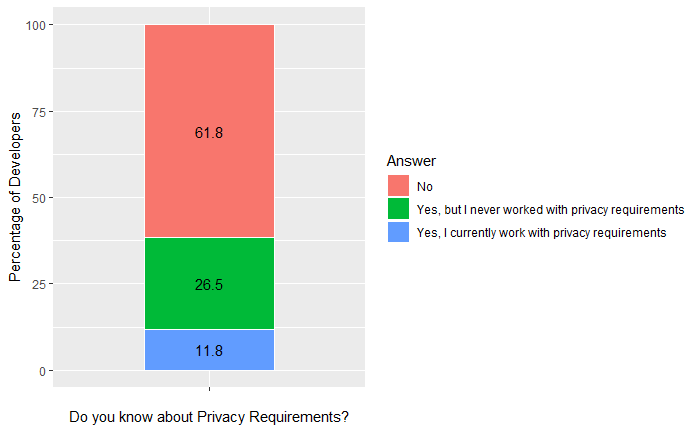
\includegraphics[width=3.5in]{Figures/RQ14.png}
    %\caption{Conhecimento dos Desenvolvedores em Relação à Privacy Requirements}
    \caption{Developers' Knowledge of Privacy Requirements}
    \label{fig:conhecimentoPR}
\end{figure}

\subsection{RQ.2. What tools related to the Empathy phase can be used to facilitate the privacy requirements elicitation?}

\todo[inline]{aqui temos que descrever as que achamos na literatura -- Eu só consegui 3 algum tem mais?}

%Ferreira et al \cite{DBLP:conf/hci/FerreiraBC16} created the PATHY technique based on both Empathy Maps and Personas, aiming to help software engineers to reflect on the users' needs. Os autores realizaram um estudo empírico para identificar a percepção dos engenheiros de software sobre a utilidade e facilidade de uso da técnica. A ferramenta PATHY foi considerado fácil de usar e útil.

Ferreira et al \cite{DBLP:conf/hci/FerreiraBC16} created the PATHY technique based on both Empathy Maps and Personas, aiming to help software engineers to reflect on the users' needs. The authors conducted an empirical study to identify the perception of software engineers about the usefulness and ease of use of the technique. The PATHY tool was found to be easy to use and useful.

%O trabalho apresentado por \cite{DBLP:conf/hci/ChasanidouGL15} utilizou a ferramenta Smaply juntamente com o Design Thinking na etapa de requirements elicitation. Os autores realizaram dois experimentos e em ambos os experimentos os participantes afirmaram que o uso da ferramenta Smaply e do Design Thinking facilitar o processo de elicitação de requisitos e permitiram uma melhor interação com os usuários.

The work presented by \cite{DBLP:conf/hci/ChasanidouGL15} used the Smaply tool together with Design Thinking in the requirements elicitation stage. The authors carried out two experiments and in both experiments the participants stated that the use of the Smaply tool and Design Thinking facilitate the process of requirements elicitation and allowed for better interaction with users.

A Web-based system referred to as \href{www.touchpointdashboard.com}{Touchpoint Dashboard} can be used for visualization of software user experience. Visual notations are used for unification of team by conversion of information into a customer journey.  This tool can be employed during the empathy phase \cite{kumar2020methods}.

%Nós investigamos se os desenvolvedores conhecem 3 das ferramentas citadas na literatura e se elas podem facilitar o processo de privacy requirements elicitation. A maioria dos desenvolvedores afirmaram não conhecer as ferramentas, conforme apresentado na Figura \ref{fig:tool}.

We investigated if the developers knew three of the tools cited in the literature and whether they can facilitate the privacy requirements elicitation process. Most developers said they did not know the tools, as shown in Figure \ref{fig:tool}.

\begin{figure}
    \centering
    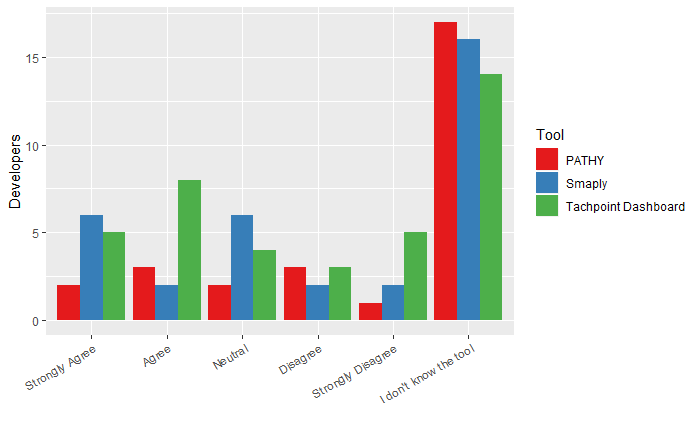
\includegraphics[width=3.5in]{Figures/RQ18.png}
    \caption{Tools related to the Empathy phase be used to facilitate the privacy requirements elicitation}
    \label{fig:tool}
\end{figure}

%Em relação as fases do Design Thinking que são consideradas mais impactantes pelos desenvolvedores na privacy requirements elicitation, 38\% dos desenvolvedores afirmaram que é a fase de Empatia, 24\% que é a fase de Definition, 16\% a fase de Ideation, 14\% a fase de prototyping and 8\% afirmaram que é a fase de Tests, conforme apresentado na Figura \ref{fig:impactos}. A partir deste resultado, podemos concluir que a fase de Empatia é considerada a fase mais importante para os desenvolvedores de software na privacy requirements elicitation. Assim, um modelo de empatia que possa ajudar os desenvolvedores na execução da atividade de requirements elicitation poderá permitir uma melhor compreensão dos requisitos e uma requirements elicitation com qualidade e menos propensa a erros.

Regarding the Design Thinking phases that are considered most impactful by the developers in the privacy requirements elicitation, 38\% of the developers stated that it is the Empathy phase, 24\% that is the Definition phase, 16\% the Ideation phase, 14\% the prototyping phase and 8\% stated that it is the Test phase, as shown in Figure \ref{fig:impacts}. From this result, we can conclude that the Empathy phase is considered the most important phase for software developers in privacy requirements elicitation. Thus, an empathy model that can help developers in the execution of the requirements elicitation activity may allow a better understanding of the requirements and a quality elicitation with less errors.

\begin{figure}
    \centering
    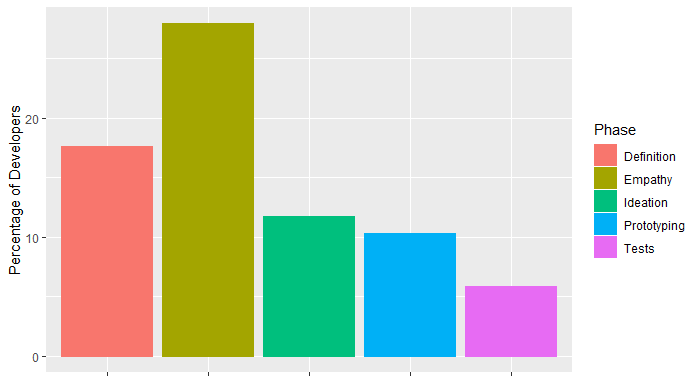
\includegraphics[width=3.5in]{Figures/RQ15.png}
    \caption{Phases of Design Thinking are most impactful in privacy requirements elicitation}
    \label{fig:impactos}
\end{figure}

\subsection{RQ.3. Is Empathy related to a skill of the software developer or to an organizational orientation (standardized/defined process by the organization)?}

%Nesta questão nós tentamos identificar a percepeção dos desenvolvedores de software em relação as habilidades de empatia, investigando se deve ser uma orientação da organização ou uma iniciativa do próprio desenvolvedor de software. Algumas respostas que nós obtivemos foram:

In this question we tried to identify the perception of software developers in relation to empathy skills, investigating whether it should be an orientation of the organization or an initiative of the software developer itself. Some answers we got were:

\begin{mq}
%\emph{"A Empatia está relacionada com a habilidade do desenvolvedor e com o processo da empresa para melhorar a requirements elicitation."}
\emph{"Empathy is related to the developer's ability and the company's process to improve requirements elicitation."}
\end{mq}

\begin{mq}
%\emph{"A empatia está relacionada a orientação organizacional (processo padronizado/definido pela organização)."}
\emph{"Empathy is related to organizational orientation (standardized/defined process by the organization)."}
\end{mq}

\begin{mq}
%\emph{"A empatia está relacionada a uma habilidade do desenvolvedor, mas seria muito importante que toda organização tivesse um processo padronizado para a atividade de requirements elicitation, inclusive com capacitação das áreas envolvidas."}
\emph{"Empathy is related to a skill of the developer, but it would be very important for every organization to have a standardized process for the activity of requirements elicitation, including training for the areas involved."}
\end{mq}

\begin{mq}
%\emph{"A fase de Empatia pode estar relacionada tanto a uma habilidade do desenvolvedor quanto a uma orientação organizacional. Todavia, por ser uma fase em que as tarefas requerem um bom entendimento de qualidade das pessoas, eu acredito que quando a iniciativa vem do desenvolvedor, os resultados alcançados durante a requirements elicitation tendem a ser mais efetivos."}
\emph{"The Empathy phase can be related to both a developer skill and an organizational orientation. However, because it is a phase in which tasks require a good understanding of people's quality, I believe that when the initiative comes from the developer, the results achieved during requirements elicitation tend to be more effective."}
\end{mq}

\begin{mq}
\emph{"I believe the organizational orientation can target a wide variety of users but without relating to most of them. In short, I believe that both approaches have strengths and weaknesses. It is up to every project leader to assign the most appropriate solution."}
\end{mq}

%De acordo com as respostas obtidas, podemos concluir que os desenvolvedores acreditam que a empatia é uma habilidade pessoal do desenvolvedor e que as organizações precisam oferecer condições para que os practitioners que não possuem essa habilidade, possam realizar treinamentos para que a atividade de requirements elicitation seja realizada com mais clareza. Esse resultado corrobora com os achados de Levy and Hadar \cite{DBLP:conf/re/LevyH18}, em que os participantes do estudo afirmaramm que a Empathy é uma habilidade do desenvolvedor e não uma orientação da organização para facilitar a elicitação de requisitos.    

According to the responses obtained, we can conclude that developers believe that empathy is a personal skill of the developer and that organizations need to offer conditions to practitioners who do not have this skill can conduct training to perform clearly the requirements elicitation activity. This result corroborates the findings of Levy and Hadar \cite{DBLP:conf/re/LevyH18}, in which the study participants stated that Empathy is a skill of the developer and not an orientation of the organization to facilitate the requirements elicitation.

\subsection{Focus Group}

\todo[inline]{aqui descreveremos os resultados com o grupo focal}

%
%\begin{figure*}[!t]
%\centering
%\subfloat[Case I]{\includegraphics[width=2.5in]{box}%
%\label{fig_first_case}}
%\hfil
%\subfloat[Case II]{\includegraphics[width=2.5in]{box}%
%\label{fig_second_case}}
%\caption{Simulation results for the network.}
%\label{fig_sim}
%\end{figure*}
%

\section{Proposed Model}
\label{empathy}
\todo[inline]{coloquei aqui para ver se conseguimos. Se não der para fazermos para o RE acho que devemos tentar para o Amcis}

%A principal diferença da proposta do nosso trabalho para o modelo PATHY é que o nosso modelo proposto será validado com desenvolvedores de software.
The main difference from the proposal of our work for the PATHY model is that our proposed model will be validated with software developers.

\section{Threats to Validity}
\label{thread}

%Como qualquer pesquisa de campo, este trabalho também possui limitações e ameaças à validade. Para conseguir atingir um número maior de participantes, o questionário foi disponibilizado em um formulário online e disseminado para diversos profissionais de empresas diferentes. Porém, devido a pesquisa não ser presencial há um risco de as pessoas preencherem sem o comprometimento necessário.

As any field research, this work also has limitations and threats to validity. In order to reach a larger number of participants, the questionnaire was made available in an online form and disseminated to several practitioners from different companies. However, the research was not in person and there was a risk that people would fill it out without the necessary commitment.

%Além disso, por um certo período de disponibilização do formulário online, o questionário estava em língua inglesa, sendo que grande parte das pessoas que preencheram eram brasileiros, o que pode ter causado ruídos de interpretação devido a alguma dificuldade com a língua estrangeira.

In addition, for a certain period of availability of the online form, the questionnaire was in English, and most of the people who filled it out were Brazilian, which may have caused interpretation noise due to some difficulty with the foreign language.

%Para efetuar a seleção do grupo focal, observamos que a maioria das empresas no Brasil ainda não estão tratando a privacidade de dados com a importância necessária, mesmo sabendo que a LGPD entrará em vigor em breve e poderá punir as empresas em caso de vazamento de dados dos usuários. Por isso, ainda não há uma definição nas empresas de quem será o responsável por levantar os requisitos de privacidade, se serão profissionais com o perfil voltado ao desenvolvimento de software, ou à segurança da informação.

In order to select the focus group, we note that most companies in Brazil are not treating data privacy with the necessary importance yet, although they know that the LGPD will come into effect soon and will be able to punish companies in case of leak of user data. For this reason, there is still no definition in companies of who will be responsible for raising privacy requirements, if they will be practitioners with a profile focused on software development, or information security.

%Contudo, conforme apresentado no resultado da pesquisa, não foi possível observar o nível de empatia no levantamento de requisitos de privacidade nas empresas devido aos profissionais não conhecerem a técnica Design Thinking e por não utilizarem ainda um processo diferente para efetuar o levantamento de requisitos de privacidade.

However, as presented in the survey result, it was not possible to observe the level of empathy in the survey of privacy requirements in companies due to practitioners not knowing the Design Thinking technique and for not yet using a different process to survey privacy requirements.

\section{Conclusion}
\label{conclusion}

\section*{Acknowledgment}

\bibliographystyle{IEEEtran}
\bibliography{paper}

\end{document}


